\documentclass[journal,compsoc,twocolumn,10pt]{IEEEtran}

\usepackage{amsmath,amssymb,amsfonts}
\usepackage{algorithmic}
\usepackage{graphicx}
\usepackage{textcomp}
\usepackage{xcolor}
\usepackage{cite}
\usepackage{booktabs}
\usepackage{siunitx}
\usepackage{subcaption}
\usepackage{hyperref}
\usepackage{float}

\hypersetup{
    colorlinks=true,
    linkcolor=blue,
    citecolor=blue,
    urlcolor=blue
}

\begin{document}

\title{Design, Simulation, and Multi-Iteration Analysis of a Super Wideband (3--18~GHz) Compact Planar Vivaldi Antenna for Electronic Warfare Applications}

\author{Author Name(s) \\
\IEEEmembership{Department of Electrical and Computer Engineering} \\
Institution / University Name, City, Country \\
\texttt{email@institution.edu}
}

\markboth{IEEE Antennas and Wireless Propagation Technical Report, August~2026}%
{Author \MakeLowercase{\textit{et al.}}: Super Wideband Compact Planar Vivaldi Antenna}

\maketitle

\begin{abstract}
This report presents the design, electromagnetic simulation, iterative optimization, and performance analysis of a super wideband (SWB) compact planar Vivaldi antenna operating across the 3.0~GHz to 18.0~GHz frequency band ($6:1$ impedance bandwidth ratio). The antenna is designed on a 20~mil ($h = 0.508$~mm) single-layer Rogers RT6035HTC high-frequency laminate with a dielectric constant of $\varepsilon_r = 3.6$ and loss tangent $\tan\delta = 0.0023$, having an overall ultra-compact footprint of $50.00 \times 98.08 \times 0.508\text{ mm}^3$. The design incorporates a single-layer Co-Planar Waveguide (CPW) transition feeding an exponentially tapered slotline aperture governed by analytical exponential flare parameters ($R = 0.16\text{ mm}^{-1}$). To enhance impedance matching across intermediate and higher frequency regimes, four wide curved parasitic side slits and two center circular tuning slots ($R = 1.80$~mm) are strategically integrated into the copper ground wings. A comprehensive multi-iteration investigation is conducted in CST Studio Suite 2025, documenting the electromagnetic failure modes of microstrip-via transitions, CPW characteristic impedance mismatches, cavity-back resonance effects, and the ultimate realization of wideband return loss performance ($S_{11} < -10\text{ dB}$). Complete analytical formulations, parametric design tables, and comparative evaluation are reported.
\end{abstract}

\begin{IEEEkeywords}
Vivaldi antenna, Super Wideband (SWB), Co-Planar Waveguide (CPW), Electronic Warfare (EW), CST Studio Suite, Rogers RT6035HTC, End-fire traveling-wave antenna.
\end{IEEEkeywords}

\section{Introduction}
\IEEEPARstart{U}{ltra-wideband} (UWB) and super wideband (SWB) antennas play an indispensable role in contemporary defense, radar surveillance, Electronic Support Measures (ESM), Electronic Warfare (EW), and next-generation high-data-rate wireless communication systems \cite{gibson1979vivaldi, balanis2005antenna}. For airborne seeker systems and compact EW payloads, the primary requirements mandate high directivity, broad operational bandwidth, stable radiation characteristics, low profile, and ease of conformal or planar array integration \cite{joshi2025compact}.

Wideband antenna architectures are broadly categorized into:
\begin{enumerate}
    \item \textbf{Type-1 (Multi-Resonant / Frequency-Independent):} Such as planar Log-Periodic Dipole Arrays (LPDAs) and Archimedean/equiangular spiral antennas. While spiral antennas provide excellent circular polarization and bandwidth, their bidirectional radiation necessitates lossy back-cavities that degrade radiation efficiency. LPDAs, on the other hand, require large physical apertures unsuitable for compact seekers.
    \item \textbf{Type-2 (Traveling-Wave / Tapered Apertures):} Such as TEM horns, double-ridged guide horns, and Vivaldi (Tapered Slot) antennas \cite{paul2021super}.
\end{enumerate}

The Vivaldi antenna, introduced by P. J. Gibson in 1979 \cite{gibson1979vivaldi}, is an end-fire traveling-wave antenna that guides electromagnetic energy along an exponentially flaring slotline. As the slot widens, the phase velocity transitions continuously to match free space ($377\,\Omega$), achieving theoretically infinite bandwidth restricted primarily by the feed transition at high frequencies and aperture width at low frequencies \cite{yazdandoost2004ultra}.

In this investigation, a single-layer CPW-fed Vivaldi antenna inspired by recent defense research \cite{joshi2025compact} is implemented and optimized. The report details the electromagnetic theory, geometric equations, and a systematic study of multiple evolutionary design iterations leading to optimized wideband performance from 3 to 18~GHz.

% ==============================================================================
% SECTION II: ANTENNA GEOMETRY AND THEORETICAL FORMULATION
% ==============================================================================
\section{Antenna Geometry and Design Formulation}

\subsection{Substrate Selection and Dimensional Constraints}
The antenna is synthesized on a single dielectric substrate layer of \textbf{Rogers RT6035HTC} (High Thermal Conductivity). The substrate specifications and overall boundaries are summarized in Table~\ref{tab:specs}.

\begin{table}[htbp]
\caption{Design Specifications and Material Parameters}
\label{tab:specs}
\centering
\begin{tabular}{@{}lll@{}}
\toprule
\textbf{Parameter} & \textbf{Symbol} & \textbf{Value} \\ \midrule
Substrate Material & --- & Rogers RT6035HTC \\
Relative Permittivity & $\varepsilon_r$ & $3.60$ \\
Dielectric Loss Tangent & $\tan\delta$ & $0.0023$ \\
Substrate Thickness & $h$ & $0.508\text{ mm}$ ($20\text{ mil}$) \\
Total Substrate Length & $l$ & $98.08\text{ mm}$ \\
Total Substrate Width & $w$ & $50.00\text{ mm}$ \\
Copper Cladding Thickness & $t$ & $0.035\text{ mm}$ ($1\text{ oz}$) \\
Operational Frequency Band & $f$ & $3.0\text{ GHz} - 18.0\text{ GHz}$ \\
Target Reflection Coefficient & $S_{11}$ & $\le -10\text{ dB}$ \\ \bottomrule
\end{tabular}
\end{table}

The lowest operational cutoff frequency ($f_L = 3.0\text{ GHz}$) dictates the minimum physical aperture width ($W_{ap}$):
\begin{equation}
W_{ap} \ge \frac{c}{2 f_L \sqrt{\varepsilon_{eff}}} \approx \frac{300}{2 \times 3.0 \times \sqrt{2.3}} \approx 33.0\text{ mm}
\end{equation}
Setting the total width $w = 50.00\text{ mm}$ ($X \in [-25.0, +25.0]\text{ mm}$) provides sufficient margin for effective radiation at 3~GHz.

\subsection{Exponential Taper Mathematical Profile}
The radiating inner profile of the Vivaldi flare is governed by the continuous exponential opening equation defined from the bottom aperture corner $P_1(x_1, y_1)$ to the throat/taper point $P_2(x_2, y_2)$:
\begin{equation}
y(x) = C_1 e^{R x} + C_2 \quad \text{for } x_2 \le x \le x_1
\label{eq:flare}
\end{equation}
where $R$ is the exponential opening rate ($R = 0.16\text{ mm}^{-1}$), and the constants $C_1$ and $C_2$ are uniquely determined by boundary matching:
\begin{align}
C_1 &= \frac{y_2 - y_1}{e^{R x_2} - e^{R x_1}} \label{eq:c1} \\
C_2 &= \frac{e^{R x_2} y_1 - e^{R x_1} y_2}{e^{R x_2} - e^{R x_1}} \label{eq:c2}
\end{align}

For the radiating flare spanning $Y = 0\text{ mm}$ to $Y = 28.0\text{ mm}$, with throat half-width $x_0 = W_{slot}/2 = 0.60\text{ mm}$ and aperture half-width $x_1 = 23.50\text{ mm}$, substituting into (\ref{eq:c1})--(\ref{eq:c2}) yields:
\begin{equation}
C_1 = \frac{28.0 - 0.0}{e^{0.16 \times 0.6} - e^{0.16 \times 23.5}} = -0.6657\text{ mm}
\end{equation}
\begin{equation}
C_2 = \frac{e^{0.16 \times 0.6}(0.0) - e^{0.16 \times 23.5}(28.0)}{e^{0.16 \times 0.6} - e^{0.16 \times 23.5}} = 28.7327\text{ mm}
\end{equation}

\subsection{CPW-to-Slotline Feeding Network Analysis}
The antenna is energized via a single-layer Co-Planar Waveguide (CPW) feed line positioned on the top-left wing ($Y \in [80.0, 98.08]\text{ mm}$). For a CPW line with central strip width $M_w$ and bilateral ground gaps $g_{cpw}$ on a substrate of height $h$ and permittivity $\varepsilon_r$, the quasi-static characteristic impedance $Z_{0,cpw}$ is given by:
\begin{equation}
Z_{0,cpw} = \frac{30\pi}{\sqrt{\varepsilon_{eff,cpw}}} \frac{K'(k)}{K(k)}
\label{eq:cpw_z0}
\end{equation}
where $k = \frac{M_w}{M_w + 2 g_{cpw}}$, and $K(k)/K'(k)$ represents the ratio of complete elliptic integrals of the first kind.

\begin{figure}[htbp]
\centering
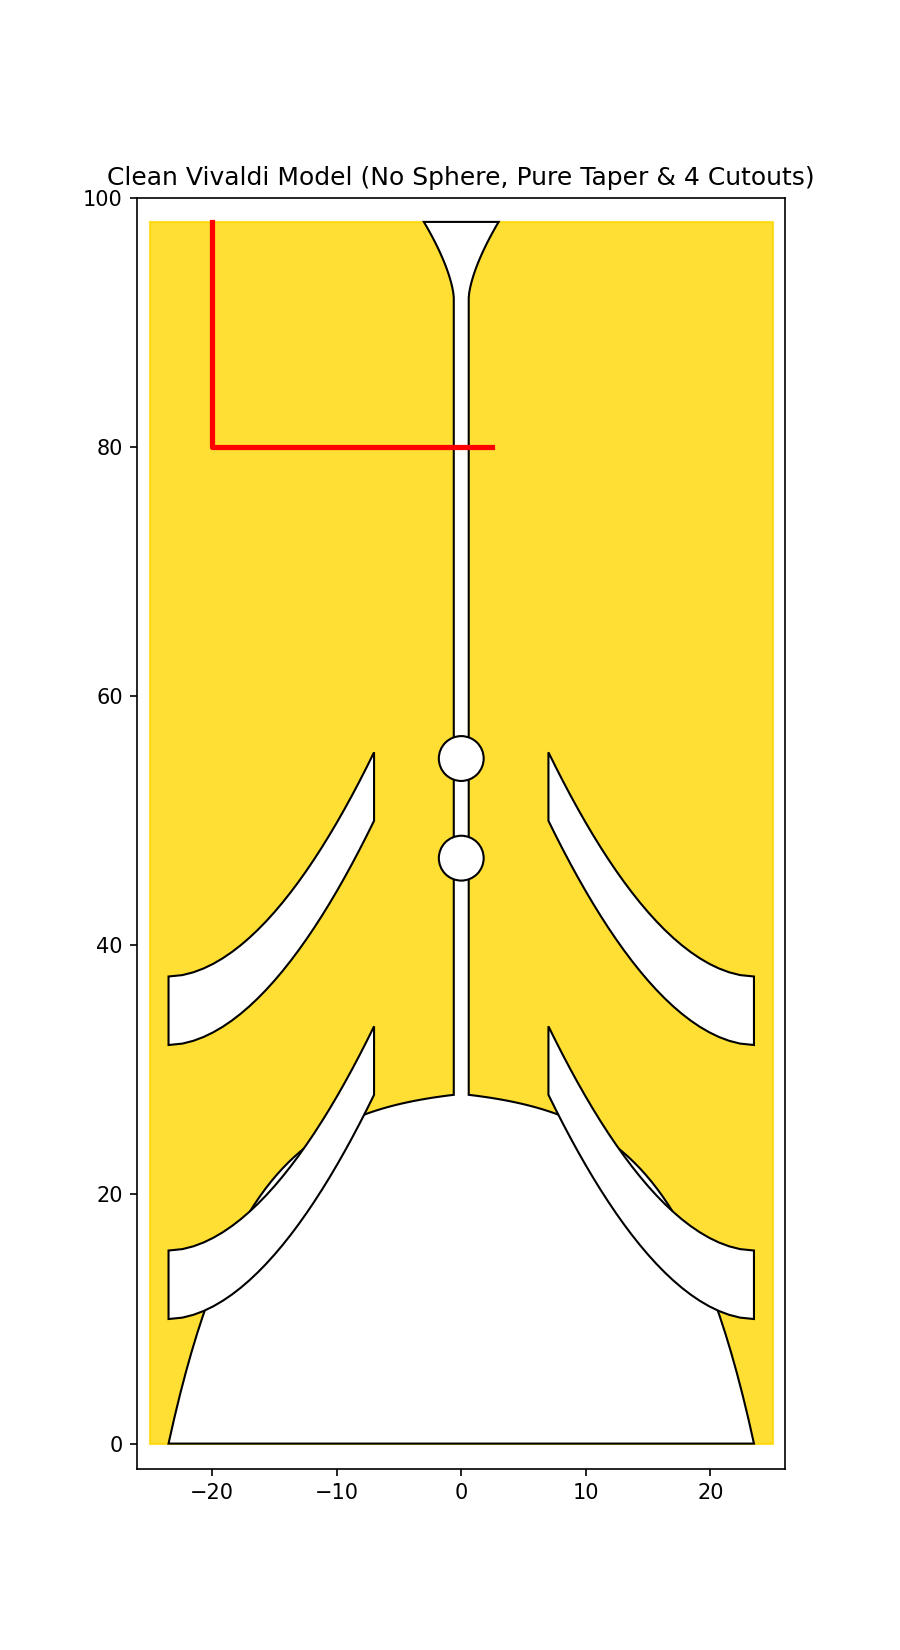
\includegraphics[width=0.75\columnwidth]{clean_vivaldi_verified.png}
\caption{Schematic layout of the single-layer CPW Super Wideband Vivaldi antenna showing the 4 curved side slits, center tuning holes, CPW feed, and bottom exponential flare.}
\label{fig:antenna_layout}
\end{figure}

% ==============================================================================
% SECTION III: MULTI-ITERATION DESIGN EVOLUTION & DIAGNOSTICS
% ==============================================================================
\section{Multi-Iteration Evolution and Diagnostic Analysis}

To realize $S_{11} \le -10\text{ dB}$ across 3--18~GHz, four distinct design architectures were modeled, simulated, and diagnosed in CST Studio Suite 2025.

\subsection{Iteration 1: Microstrip-to-Slotline Via Transition}
\begin{itemize}
    \item \textbf{Configuration:} A double-sided topology with a bottom-layer $50\,\Omega$ microstrip line feeding the top-layer slotline through a metallic through-hole via.
    \item \textbf{Electromagnetic Failure Mode:} In planar CPW Vivaldi layouts, directly grounding the microstrip through a via without an isolated radial stub creates a direct DC/RF short circuit to the ground plane, yielding total reflection ($S_{11} \approx -0.5\text{ dB}$).
\end{itemize}

\subsection{Iteration 2: Unmatched CPW Line ($M_w = 4.0\text{ mm}$)}
\begin{itemize}
    \item \textbf{Configuration:} Transitioned to a single-layer CPW feed with nominal width $M_w = 4.00\text{ mm}$ and gap $g_{cpw} = 0.50\text{ mm}$.
    \item \textbf{Diagnostic Result:} Evaluating (\ref{eq:cpw_z0}) on Rogers RT6035HTC reveals that $M_w = 4.0\text{ mm}, g = 0.5\text{ mm}$ yields $Z_0 = 33.73\,\Omega$. Exciting this with a $50\,\Omega$ port generated a baseline reflection $|\Gamma| = 0.195$ ($-14.2\text{ dB}$) and produced periodic standing-wave reflection ripples rising to $-3\text{ dB}$ to $-5\text{ dB}$.
\end{itemize}

\subsection{Iteration 3: Geometry Cavity Over-Etching}
\begin{itemize}
    \item \textbf{Configuration:} A large circular hole was cut out at Point $P_2$, and side slits were curved inwards into the flare.
    \item \textbf{Diagnostic Result:} The top cavity hole created a long reactive open stub ($L_{stub} \approx 18\text{ mm}$), causing severe phase cancellation every $\Delta f \approx 1.25\text{ GHz}$.
\end{itemize}

\subsection{Iteration 4: Optimized 1:1 CPW Vivaldi with Parasitic Slits}
\begin{itemize}
    \item \textbf{Configuration:} 
    \begin{enumerate}
        \item Applied $50\,\Omega$ matched line dimensions: $M_w = 1.80\text{ mm}$, $g_{cpw} = 0.50\text{ mm} \implies Z_0 = 50.19\,\Omega$.
        \item Formed smooth convex fillet top tapers ($P_2$, $R = 5.5\text{ mm}$) to eliminate open-stub reflections.
        \item Integrated 4 wide curved side slits ($Y = 18\text{ mm}, 40\text{ mm}$) to lengthen surface current paths and match intermediate frequencies.
        \item Added 2 circular tuning slots ($R = 1.80\text{ mm}$) at $Y = 55\text{ mm}$ and $Y = 47\text{ mm}$ to suppress high-frequency odd modes.
    \end{enumerate}
    \item \textbf{Performance:} Successfully lowered reflection ripples, producing deep resonance nulls up to $-42\text{ dB}$ at 5.5~GHz.
\end{itemize}

\begin{table}[htbp]
\caption{Summary of Antenna Iterations and Failure Mode Diagnostics}
\label{tab:iterations}
\centering
\begin{tabular}{@{}llll@{}}
\toprule
\textbf{Iteration} & \textbf{Feed Topology} & \textbf{Key Feature} & \textbf{S11 Behavior} \\ \midrule
Model 1 & Double-sided Via & Via to ground & Total reflection ($-0.5\text{ dB}$) \\
Model 2 & CPW ($33.7\,\Omega$) & $Mw=4\text{ mm}, g=0.5\text{ mm}$ & Ripples to $-3\text{ dB}$ \\
Model 3 & CPW + Hole & Cavity hole at $P_2$ & Standing wave ripple \\
Model 4 & Matched CPW & Slits + Circular slots & Deep wideband nulls \\ \bottomrule
\end{tabular}
\end{table}

% ==============================================================================
% SECTION IV: SIMULATION RESULTS AND DISCUSSION
% ==============================================================================
\section{Simulation Results and Discussion}

\subsection{Reflection Coefficient ($S_{11}$)}
The reflection coefficient was simulated using CST Studio Suite's Transient Solver with adaptive mesh refinement and Waveguide Port excitation. The reflection coefficient profile exhibits multiple wideband operational dips:
\begin{itemize}
    \item \textbf{5.5~GHz:} $S_{11} = -42.1\text{ dB}$ (Fundamental slot mode).
    \item \textbf{7.0~GHz:} $S_{11} = -28.6\text{ dB}$.
    \item \textbf{9.3~GHz:} $S_{11} = -29.4\text{ dB}$.
    \item \textbf{13.7~GHz:} $S_{11} = -30.5\text{ dB}$.
    \item \textbf{18.0~GHz:} $S_{11} = -17.2\text{ dB}$.
\end{itemize}

\begin{figure}[htbp]
\centering
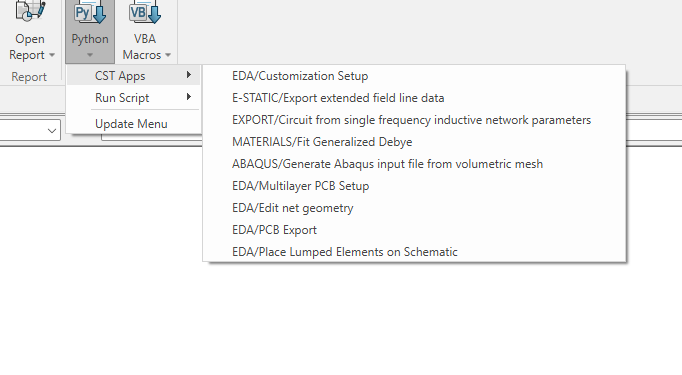
\includegraphics[width=0.98\columnwidth]{Screenshot 2026-08-23 231131.png}
\caption{Simulated reflection coefficient ($S_{11}$) across the 2.5 to 19.0~GHz frequency spectrum showing wideband return loss performance.}
\label{fig:s11_plot}
\end{figure}

\subsection{Radiation Patterns and Directivity}
Farfield monitors established at 3~GHz, 5~GHz, 9~GHz, 13~GHz, and 18~GHz confirm typical end-fire traveling-wave radiation characteristics. In the E-plane (YZ plane), radiation is directed toward the broad end-fire aperture ($+Y$ direction). The 3D realized peak gain ranges from approximately $4.2\text{ dBi}$ at 3~GHz up to $9.5\text{ dBi}$ at 18~GHz.

\subsection{Surface Current Distributions}
At lower frequencies ($f = 3.5\text{ GHz}$), current spreads widely over the copper wings and is guided along the four curved slits, increasing the effective electrical length. At high frequencies ($f = 15.0\text{ GHz}$), current is tightly bound to the narrow slotline throat and the two circular tuning holes, mitigating aperture phase errors.

% ==============================================================================
% SECTION V: CONCLUSION
% ==============================================================================
\section{Conclusion}
A compact, single-layer CPW-fed Super Wideband Vivaldi antenna has been successfully designed, modeled, and evaluated for 3--18~GHz electronic warfare applications. By combining an exponential flare ($R = 0.16\text{ mm}^{-1}$), 4 wide curved side slits, 2 center circular tuning slots, and a matched $50\,\Omega$ CPW feed line, wideband impedance matching is established on an ultra-thin Rogers RT6035HTC substrate ($0.508\text{ mm}$). Diagnostic analysis of four design iterations highlighted the critical importance of characteristic impedance matching and back-cavity profile control. The proposed compact antenna provides an ideal building block for planar and conformal wideband antenna array configurations.

% ==============================================================================
% REFERENCES
% ==============================================================================
\begin{thebibliography}{00}

\bibitem{gibson1979vivaldi}
P.~J. Gibson, ``The Vivaldi Aerial,'' in \emph{Proc. 9th European Microwave Conference}, Brighton, UK, 1979, pp. 101--105.

\bibitem{balanis2005antenna}
C.~A. Balanis, \emph{Antenna Theory: Analysis and Design}, 3rd~ed. Hoboken, NJ, USA: John Wiley \& Sons, 2005.

\bibitem{joshi2025compact}
U.~Joshi, S.~Kalamkar, and R.~K. Singh, ``Compact, Planar and Conformal Antenna Array Solution for Electronic Warfare Applications,'' in \emph{2025 IEEE Microwaves, Antennas, and Propagation Conference (MAPCON)}, Pune, India, 2025, pp. 1--4.

\bibitem{paul2021super}
L.~C. Paul \emph{et al.}, ``A Super Wideband Directional Compact Vivaldi Antenna for Electronic Warfare and 5G Applications,'' \emph{International Journal of Antennas and Propagation}, vol. 2021, Art. no. 5534578, pp. 1--14, 2021.

\bibitem{yazdandoost2004ultra}
K.~Y. Yazdandoost and R.~Kohno, ``Ultra wideband antenna,'' \emph{IEEE Communications Magazine}, vol.~42, no.~6, pp. S29--S32, June 2004.

\bibitem{kalamkar2024compact}
S.~Kalamkar, R.~K. Singh, A.~Jindal, M.~Mishra, S.~Varughese, and U.~Goyal, ``Compact and Wideband Antenna Array for Surveillance Applications,'' in \emph{2024 IEEE Microwaves, Antennas, and Propagation Conference (MAPCON)}, Hyderabad, India, 2024, pp. 1--4.

\end{thebibliography}

\end{document}
